\section{独立部分和}
\label{sec:lln-partial-sums}

全章固定一个概率空间$(\Omega,\mathcal{F},\mathbb{P})$，在上面取一列随机变量$X_1,X_2,\dots$，并假设它们相互独立：其中任意有限个都相互独立。按第~\ref{chap:probability-spaces}章的结论，这些变量的函数，只要所用的下标组互不相交，也相互独立。例如$X_1+X_2$与$X_3X_4$独立，前$k$项的任何函数与第$k+1$项以后有限项的任何函数独立。

把前$n$项依次加起来，就得到一个随机的累计量。固定一个样本点$\omega$，$n\mapsto X_1(\omega)+\dots+X_n(\omega)$是一个普通的实数列，可以画成一条折线，每一步增加一个独立的增量。本章的所有问题都问这条折线的长期行为：它本身是否停在某处，或者除以步数以后是否停在某处。

\subsection{中心化与归一化}
\label{sec:lln-normalization}

同一列累计和可以按三种方式观察，它们回答的问题不同，先把记号定下来。

\begin{definition}[部分和、中心化部分和与样本平均]
\label{def:lln-partial-sums}
设$X_1,X_2,\dots$可积，记$\mu_k=\mathbb{E}[X_k]$。对$n\geq1$，令
\begin{equation}
 \begin{gathered}
 S_n=\sum_{k=1}^{n}X_k,\qquad \bar{X}_n=\frac{S_n}{n},\\
 \tilde{S}_n=\sum_{k=1}^{n}(X_k-\mu_k)=S_n-\mathbb{E}[S_n],
 \end{gathered}
 \label{eq:lln-partial-sums}
\end{equation}
并约定$S_0=\tilde{S}_0=0$。分别称$S_n$、$\tilde{S}_n$、$\bar{X}_n$为\term{部分和}（partial sum）、\term{中心化部分和}（centered partial sum）与\term{样本平均}（sample average）。
\end{definition}

$\mathbb{E}[S_n]=\sum_{k\leq n}\mu_k$用的是期望的线性性，下一小节再细看。部分和$S_n$收敛到有限极限，就是随机级数$\sum_kX_k$收敛，这是关于无限累计本身的问题。中心化部分和$\tilde{S}_n$去掉了各项的平均漂移，只剩随机波动；它是否收敛，问的是波动的累计能否停下来。样本平均$\bar{X}_n$把累计量按步数摊平，问的是每一步的平均贡献是否稳定。

\paragraph{同一列变量的不同答案}
取$X_k=\varepsilon_k$，其中$\varepsilon_1,\varepsilon_2,\dots$独立，各以$1/2$的概率取$+1$和$-1$。这样的$\varepsilon_k$称为随机符号，后文反复使用。这时$\mu_k=0$，三种部分和中前两种相同。$S_n$不可能收敛：相邻两项总相差$\lvert S_{n+1}-S_n\rvert=1$，对每个样本点都不是Cauchy列。平均$\bar{X}_n=S_n/n$却表现得很安稳。

图~\ref{fig:lln-three-normalizations}画出同一组五条路径的两种观察。图(a)中$S_n$在零的两侧来回游荡，偏离的典型大小与紫色虚线$\pm\sqrt{n}$同阶；图(b)中把同样的路径除以$n$，波动按$1/\sqrt{n}$收窄。下一小节会说明$\sqrt{n}$与$1/\sqrt{n}$分别是$S_n$与$\bar{X}_n$的标准差。

\begin{BookInlineFigure}
 \centering
 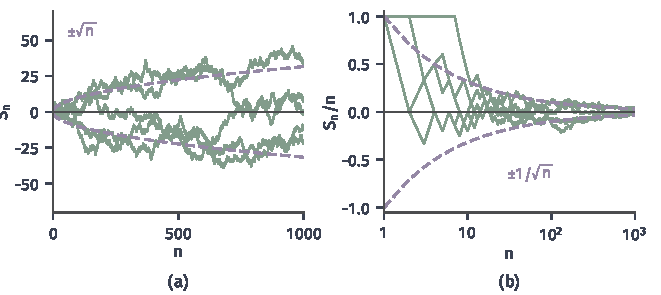
\includegraphics[width=112mm]{figures/07-probability/03-probability-limits/matplotlib/lln-three-normalizations/figure.pdf}
 \caption{随机符号的部分和与样本平均，五条路径（种子$7$）。(a)部分和$S_n$（绿线）与$\pm\sqrt{n}$（紫色虚线），横轴为线性刻度；(b)样本平均$S_n/n$（绿线）与$\pm1/\sqrt{n}$（紫色虚线），横轴为对数刻度。}
 \label{fig:lln-three-normalizations}
\end{BookInlineFigure}

反过来，给每一项加上递减的权重，累计也可能收敛。下一节将证明$\sum_k\varepsilon_k/k$几乎必然收敛，而$\sum_k\varepsilon_k/\sqrt{k}$几乎必然发散。级数问题与平均问题都由部分和出发，但所用的尺度不同，结论也就不同。

\paragraph{各项均值不同时}
当$X_k$不同分布时，各项均值$\mu_k$可以互不相同，中心化必须逐项减去自己的$\mu_k$。如果$\mu_k$的平均本身不收敛，就不存在一个共同的数可以作为$\bar{X}_n$的极限。

看一个具体的例子。令$X_k\sim\operatorname{Bern}(p_k)$相互独立，其中
\[
 p_k=\begin{cases}0.2, & 2^j\leq k<2^{j+1},\ j\ \text{为偶数},\\ 0.8, & 2^j\leq k<2^{j+1},\ j\ \text{为奇数}.\end{cases}
\]
第$j$段含$2^j$项，比前面所有段的项数之和还多一项，所以每走完一段，前$n$项均值的平均
\[
 m_n=\frac{1}{n}\sum_{k=1}^{n}p_k
\]
就被最后一段拉向它自己的取值。

具体算一下极限点。在第$J$段末尾$n=2^{J+1}-1$处，最后一段约占全部项数的$1/2$，倒数第二段约占$1/4$，依此类推。$J$为奇数时，取$0.8$的段占比约为$1/2+1/8+\dots=2/3$，于是
\[
 m_n\to0.8\cdot\tfrac23+0.2\cdot\tfrac13=0.6 ;
\]
$J$为偶数时两种取值的占比对调，$m_n\to0.4$。所以$m_n$在$0.4$与$0.6$之间往复，没有极限。

图~\ref{fig:lln-varying-means}(a)中蓝线是$m_n$，绿线是一条样本路径的$S_n/n$，后者紧跟前者摆动；图(b)画出两者之差$(S_n-\sum_{k\leq n}p_k)/n=\tilde{S}_n/n$，它趋于零。正确的问题因此是$\tilde{S}_n/n\to0$，而不是“$\bar{X}_n$趋于某个共同期望”。第~\ref{sec:lln-series-to-average}小节将证明，对这个例子$\tilde{S}_n/n$几乎必然趋于零。

\begin{BookInlineFigure}
 \centering
 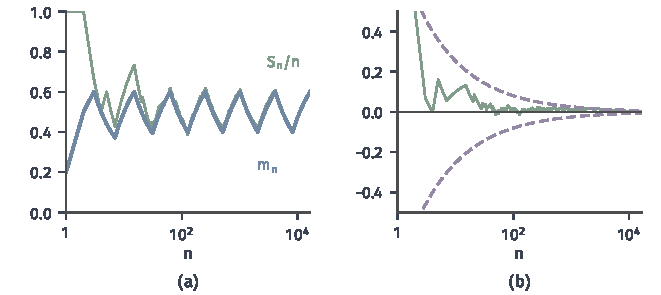
\includegraphics[width=112mm]{figures/07-probability/03-probability-limits/matplotlib/lln-varying-means/figure.pdf}
 \caption{分段取均值的独立Bernoulli变量，$p_k$在长度倍增的各段上交替取$0.2$与$0.8$，一条路径（种子$3$），横轴为对数刻度。(a)均值的平均$m_n$（蓝线）与样本平均$S_n/n$（绿线）；(b)差$(S_n-\sum_{k\leq n}p_k)/n$（绿线）与两倍标准差包络（紫色虚线）。}
 \label{fig:lln-varying-means}
\end{BookInlineFigure}

\subsection{均值与方差}
\label{sec:lln-mean-variance}

要判断累计量的走向，先看它在一个固定终点$n$处的中心和散布。中心由期望给出，不需要独立；散布由方差给出，独立性在这里第一次起作用。

\begin{theorem}[独立和的均值与方差]
\label{thm:lln-mean-variance}
设$X_1,\dots,X_n$可积，$\mu_k=\mathbb{E}[X_k]$。则
\begin{equation}
 \mathbb{E}[S_n]=\sum_{k=1}^{n}\mu_k .
 \label{eq:lln-sum-mean}
\end{equation}
若进一步$X_1,\dots,X_n$相互独立，且$\sigma_k^2=\operatorname{Var}(X_k)<\infty$，则
\begin{equation}
 \operatorname{Var}(S_n)=\mathbb{E}[\tilde{S}_n^2]=\sum_{k=1}^{n}\sigma_k^2 .
 \label{eq:lln-sum-variance}
\end{equation}
式~\eqref{eq:lln-sum-variance}只用到两两不相关，即$j\neq k$时$\operatorname{Cov}(X_j,X_k)=0$。
\end{theorem}

\begin{proof}
式~\eqref{eq:lln-sum-mean}是期望的线性性。对方差，记$D_k=X_k-\mu_k$，则$\tilde{S}_n=\sum_kD_k$。把平方展开成对角项与交叉项：
\[
 \tilde{S}_n^2=\sum_{k=1}^{n}D_k^2+\sum_{j\neq k}D_jD_k .
\]
由$\lvert D_jD_k\rvert\leq(D_j^2+D_k^2)/2$，每个交叉项都可积。$X_j$与$X_k$独立时，$D_j$与$D_k$也独立，乘积的期望等于期望的乘积，见第~\ref{chap:random-vectors}章，于是
\[
 \mathbb{E}[D_jD_k]=\mathbb{E}[D_j]\,\mathbb{E}[D_k]=0\cdot0=0 .
\]
对展开式取期望，交叉项全部消失，剩下$\sum_k\mathbb{E}[D_k^2]=\sum_k\sigma_k^2$。这一步只用了$\mathbb{E}[D_jD_k]=\operatorname{Cov}(X_j,X_k)=0$。
\end{proof}

\paragraph{波动为什么只按平方根增长}
把方差看作质量绕重心的转动惯量。独立的偏差有正有负，互相部分抵消，所以$n$项的总转动惯量只是各项之和，而不是像同向偏差那样按$n^2$增长。对比极端的相关情形：若$X_k=X_1$对所有$k$成立，则$S_n=nX_1$，方差为$n^2\sigma_1^2$。独立同分布、方差为$\sigma^2$时，式~\eqref{eq:lln-sum-variance}给出
\[
 \operatorname{Var}(S_n)=n\sigma^2,\qquad \operatorname{Var}(\bar{X}_n)=\frac{\sigma^2}{n} .
\]
部分和的标准差是$\sqrt{n}\,\sigma$，样本平均的标准差是$\sigma/\sqrt{n}$，这正是图~\ref{fig:lln-three-normalizations}中两条包络的来历。

\paragraph{固定终点的偏差}
对中心化部分和用第~\ref{chap:tail-probabilities}章的Chebyshev不等式，就得到终点处偏差的概率上界：对每个$a>0$，
\begin{equation}
 \mathbb{P}\bigl(\lvert\tilde{S}_n\rvert\geq a\bigr)\leq\frac{1}{a^2}\sum_{k=1}^{n}\sigma_k^2 .
 \label{eq:lln-endpoint-chebyshev}
\end{equation}

用骰子检验一下。掷$n=100$次均匀骰子，单次点数的方差为$35/12$，所以
\[
 \operatorname{Var}(S_{100})=100\cdot\frac{35}{12}=\frac{875}{3}\approx291.7 .
\]
取$a=30$，式~\eqref{eq:lln-endpoint-chebyshev}给出
\[
 \mathbb{P}\bigl(\lvert S_{100}-350\rvert\geq30\bigr)\leq\frac{291.7}{900}\approx0.324 .
\]
用$200000$条模拟路径（种子$12$）估计，左边约为$0.085$。界偏大，但它对任何方差为$35/12$的独立同分布序列都成立。

\paragraph{终点控制不住整段路径}
式~\eqref{eq:lln-endpoint-chebyshev}只管时刻$n$。部分和可以先越过$\pm a$，再回到区间内部。图~\ref{fig:lln-endpoint-vs-path}画出$30$条骰子路径（种子$11$），其中$4$条在$k\leq100$的某一步越过了$\pm30$，有$3$条到$k=100$时又回到了带内。模拟估计全程越过的概率约为$0.147$，比终点越过的$0.085$大不少。

\begin{BookInlineFigure}
 \centering
 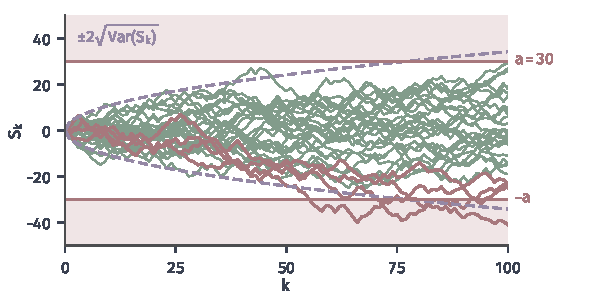
\includegraphics[width=100mm]{figures/07-probability/03-probability-limits/matplotlib/lln-endpoint-vs-path/figure.pdf}
 \caption{中心化骰子部分和$S_k=\sum_{i\leq k}(D_i-3.5)$的$30$条路径（种子$11$），$k\leq100$。红色水平线为阈值$\pm30$，浅红区域为越界区域；红线是在某一步越过阈值的路径，绿线是始终未越过的路径；紫色虚线为$\pm2\sqrt{\operatorname{Var}(S_k)}$。}
 \label{fig:lln-endpoint-vs-path}
\end{BookInlineFigure}

一个朴素的补救是对每个$k\leq n$分别用Chebyshev不等式再相加。独立同分布、方差为$\sigma^2$时，
\[
 \mathbb{P}\Bigl(\max_{k\leq n}\lvert\tilde{S}_k\rvert\geq a\Bigr)\leq\sum_{k=1}^{n}\frac{\operatorname{Var}(S_k)}{a^2}=\frac{\sigma^2}{a^2}\cdot\frac{n(n+1)}{2} .
\]
骰子例子中右边约为$16.4$，远大于$1$，毫无用处。各个时刻的越界事件高度重叠，相加把同一块概率计算了许多次。下一小节说明，对独立中心化的和，整段路径的最大偏离与终点偏差满足同一个上界。

\subsection{Kolmogorov最大不等式}
\label{sec:lln-maximal-inequality}

先猜一下最大偏离应当满足怎样的界。一条路径若在某一步$k$首次越过$a$，此后的增量既独立于过去，平均又为零，没有系统地把路径拉回来的倾向。所以终点平方的期望至少还保留着越界时的$S_k^2\geq a^2$。这就是说，越过阈值的路径不会因为“回头”而在终点的方差中消失。

\begin{theorem}[Kolmogorov最大不等式]
\label{thm:lln-kolmogorov-maximal}
设$X_1,\dots,X_n$相互独立，$\mathbb{E}[X_k]=0$，$\mathbb{E}[X_k^2]<\infty$。则对每个$a>0$，
\begin{equation}
 \mathbb{P}\Bigl(\max_{1\leq k\leq n}\lvert S_k\rvert\geq a\Bigr)\leq\frac{\operatorname{Var}(S_n)}{a^2}=\frac{1}{a^2}\sum_{k=1}^{n}\mathbb{E}[X_k^2] .
 \label{eq:lln-kolmogorov-maximal}
\end{equation}
\end{theorem}

这个不等式称为\term{Kolmogorov最大不等式}（Kolmogorov's maximal inequality）。它的右边与终点的Chebyshev界~\eqref{eq:lln-endpoint-chebyshev}完全相同，左边却换成了整段路径的最大值。

\begin{proof}
按首次越过阈值的时刻把事件拆开。对$k=1,\dots,n$，令
\[
 A_k=\bigl\{\lvert S_k\rvert\geq a,\ \lvert S_j\rvert<a\ \text{对所有}\ j<k\bigr\} .
\]
$A_k$表示“在第$k$步首次越过”。这些事件两两不交，它们的并恰为$A=\{\max_{k\leq n}\lvert S_k\rvert\geq a\}$。

由于$S_n^2\geq0$，且$A_1,\dots,A_n$不交，
\[
 \mathbb{E}[S_n^2]\geq\mathbb{E}[S_n^2\mathbf{1}_{A}]=\sum_{k=1}^{n}\mathbb{E}[S_n^2\mathbf{1}_{A_k}] .
\]
固定$k$，把终点写成首次越过时的位置加上之后的增量，$S_n=S_k+(S_n-S_k)$。展开平方并丢掉非负项$(S_n-S_k)^2$，得到
\[
 S_n^2\geq S_k^2+2S_k(S_n-S_k) .
\]

关键是交叉项的期望为零。$S_k\mathbf{1}_{A_k}$只依赖$X_1,\dots,X_k$，$S_n-S_k=X_{k+1}+\dots+X_n$只依赖后面的变量，两者独立，并且都平方可积。于是
\[
 \mathbb{E}\bigl[S_k\mathbf{1}_{A_k}(S_n-S_k)\bigr]=\mathbb{E}[S_k\mathbf{1}_{A_k}]\,\mathbb{E}[S_n-S_k]=0 .
\]

把上面的不等式乘以$\mathbf{1}_{A_k}$再取期望，交叉项消失。再利用$A_k$上$S_k^2\geq a^2$，得到
\[
 \mathbb{E}[S_n^2\mathbf{1}_{A_k}]\geq\mathbb{E}[S_k^2\mathbf{1}_{A_k}]\geq a^2\,\mathbb{P}(A_k) .
\]
对$k$求和，并利用$A_1,\dots,A_n$不交，得到
\[
 \mathbb{E}[S_n^2]\geq a^2\sum_{k=1}^{n}\mathbb{P}(A_k)=a^2\,\mathbb{P}(A) .
\]
最后由式~\eqref{eq:lln-sum-variance}，左边等于$\operatorname{Var}(S_n)=\sum_k\mathbb{E}[X_k^2]$，两边除以$a^2$即得。
\end{proof}

图~\ref{fig:lln-first-passage}把证明中的分解画了出来。首次越过时刻$k$之前的信息决定了$A_k$与$S_k$，之后的增量与它们独立且平均为零。路径越界后可能回到带内，但这种回头只是随机的，平均来说不抵消越界时已有的$S_k^2$。

\begin{BookInlineFigure}
 \centering
 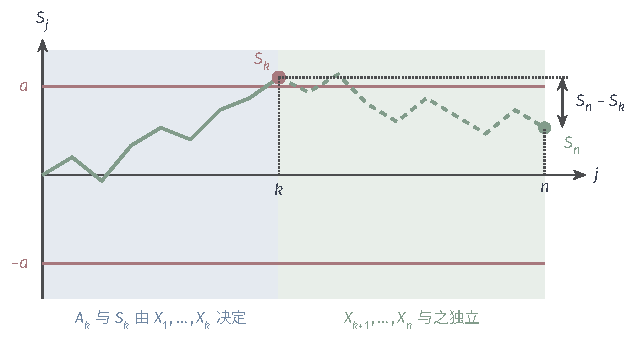
\includegraphics[width=107mm]{figures/07-probability/03-probability-limits/tikz/lln-first-passage/figure.pdf}
 \caption{Kolmogorov最大不等式的首次越过分解（示意）。绿色折线为部分和路径，在第$k$步首次达到$\lvert S_k\rvert\geq a$（红点）；浅蓝区域内的信息决定事件$A_k$，浅绿区域内的增量$X_{k+1},\dots,X_n$与之独立；终点$S_n=S_k+(S_n-S_k)$可以回到阈值以内。}
 \label{fig:lln-first-passage}
\end{BookInlineFigure}

\paragraph{一个能逐条数清的例子}
取四个随机符号，$S_k=\varepsilon_1+\dots+\varepsilon_k$，共有$2^4=16$条等可能的路径，阈值取$a=3$。图~\ref{fig:lln-rademacher-lattice}在每个节点标出经过它的路径条数。要在四步内达到$\lvert S_k\rvert\geq3$，必须前三步同号，到达$(3,\pm3)$；从那里第四步可上可下，所以共有$2\times2=4$条路径越界。终点满足$\lvert S_4\rvert\geq3$的只有终点为$\pm4$的$2$条。

\begin{BookInlineFigure}
 \centering
 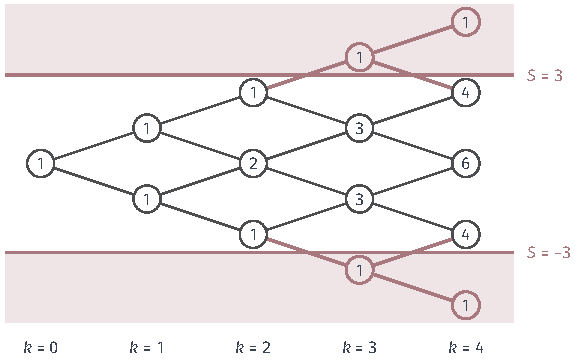
\includegraphics[width=98mm]{figures/07-probability/03-probability-limits/tikz/lln-rademacher-lattice/figure.pdf}
 \caption{四个随机符号的全部$16$条路径。节点中的数字是经过该节点的路径条数；红色水平线为$S=\pm3$，红色边与红框节点标出在某一步达到$\lvert S_k\rvert\geq3$的$4$条路径，其中$2$条在第四步回到$\pm2$。}
 \label{fig:lln-rademacher-lattice}
\end{BookInlineFigure}

于是三个量分别是
\[
 \begin{gathered}
 \mathbb{P}\Bigl(\max_{k\leq4}\lvert S_k\rvert\geq3\Bigr)=\frac{4}{16}=0.25,\qquad
 \mathbb{P}(\lvert S_4\rvert\geq3)=\frac{2}{16}=0.125,\\
 \frac{\operatorname{Var}(S_4)}{3^2}=\frac49\approx0.444 .
 \end{gathered}
\]
最大偏离的概率是终点概率的两倍，仍在Kolmogorov界之下。若取$a=2$，同样计数得到$0.75$、$0.625$与界$1$。

\paragraph{较长的路径}
图~\ref{fig:lln-maximal-compare}对$n=100$个随机符号精确计算两种概率：终点概率由二项分布求和，全程最大值越界的概率由逐步递推（越界即吸收）求得。$a=20$时终点概率为$0.057$，全程概率为$0.092$，Kolmogorov界为$0.25$，逐点相加的界却是$12.6$。Kolmogorov界与真实值的差距来自它只用了方差；真正的尾部还要轻得多，那是第~\ref{chap:central-limit-theorem}章的内容。

\begin{BookInlineFigure}
 \centering
 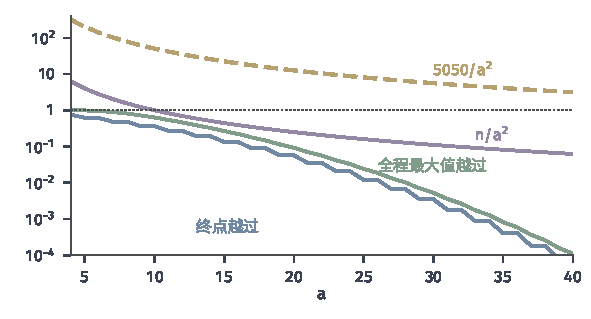
\includegraphics[width=100mm]{figures/07-probability/03-probability-limits/matplotlib/lln-maximal-compare/figure.pdf}
 \caption{$n=100$个随机符号，越界概率随阈值$a$的变化，纵轴为对数刻度。蓝线为终点概率$\mathbb{P}(\lvert S_n\rvert\geq a)$，绿线为全程最大值概率$\mathbb{P}(\max_{k\leq n}\lvert S_k\rvert\geq a)$，二者均为精确值；紫线为Kolmogorov界$n/a^2$，黄色虚线为逐点相加的界$\sum_{k\leq n}k/a^2=5050/a^2$，点线标出概率$1$。}
 \label{fig:lln-maximal-compare}
\end{BookInlineFigure}

\paragraph{条件各起什么作用}
中心化不可省略。若$X_k\equiv1$，方差为零，式~\eqref{eq:lln-kolmogorov-maximal}右边为$0$，而$\max_{k\leq n}\lvert S_k\rvert=n$。证明中用到的是$\mathbb{E}[S_n-S_k]=0$：有漂移时，越界之后的路径会被系统地推向一侧，平方的期望不再只由方差决定。

独立性也不可省略，它保证了交叉项的期望为零。取$X_1=\varepsilon_1$，$X_2=-\varepsilon_1$，两项都中心化且方差为$1$，但$S_2=0$，右边为$0$；左边在$a=1$时却等于$\mathbb{P}(\lvert S_1\rvert\geq1)=1$。这里第二步完全由第一步决定，越界后被确定地拉了回来。

这个不等式是本章的主要工具。下一节用它控制随机级数的尾段，第~\ref{sec:lln-strong-law}节再经由级数得到强大数律。
